\chapter{Boats}

Engineers have been building boats for centuries.  Through boat design, humanity learned the lessons that made airplanes and rockets possible.  
Learning about how boats work will give you a foundation for understanding more advanced concepts we will be covering later.

\section{Basic Terminology}

The front of a boat is called \newterm{the bow} (pronounced exactly the same as "bough"). The back of the boat is called \newterm{the stern}.

The underside of the boat is called \newterm{the hull}.  The top of the boat is called \newterm{the deck}.

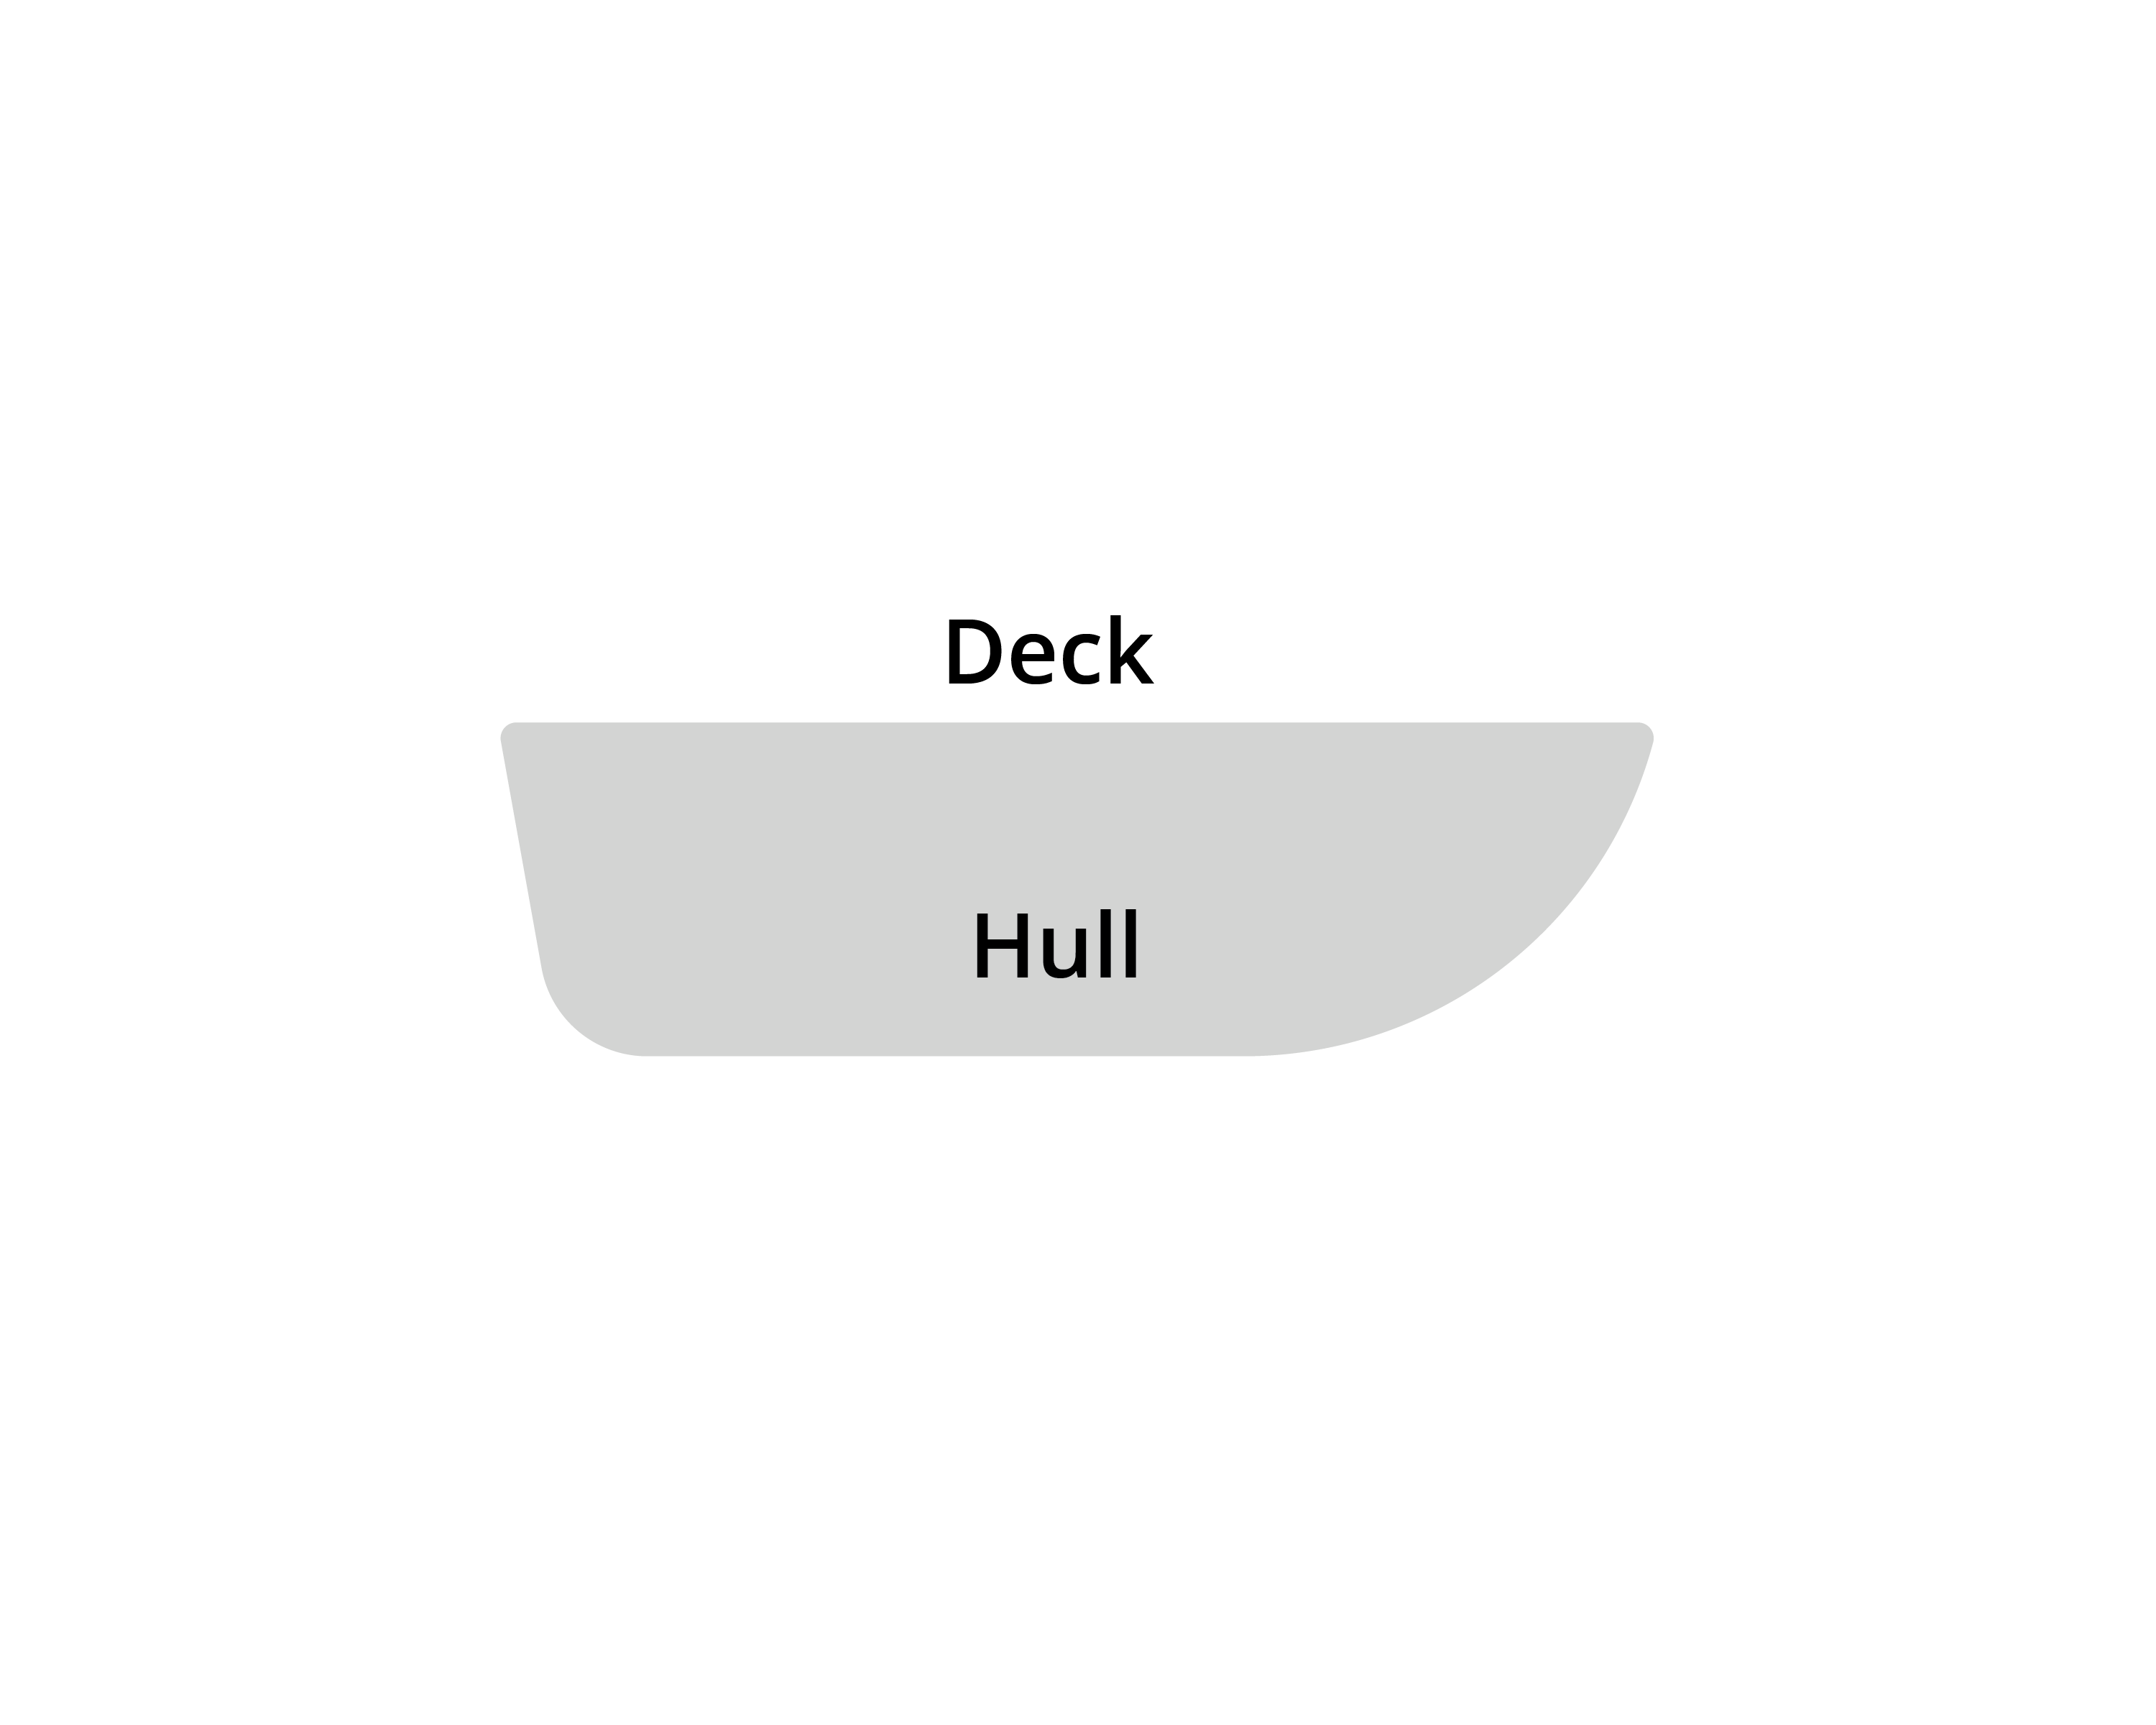
\includegraphics[width=.75\textwidth]{deckHull.png}


If you are standing at the stern and looking toward the bow, everything on your left is the \newterm{port} side.  Everything on your right is the \newterm{starboard} side.

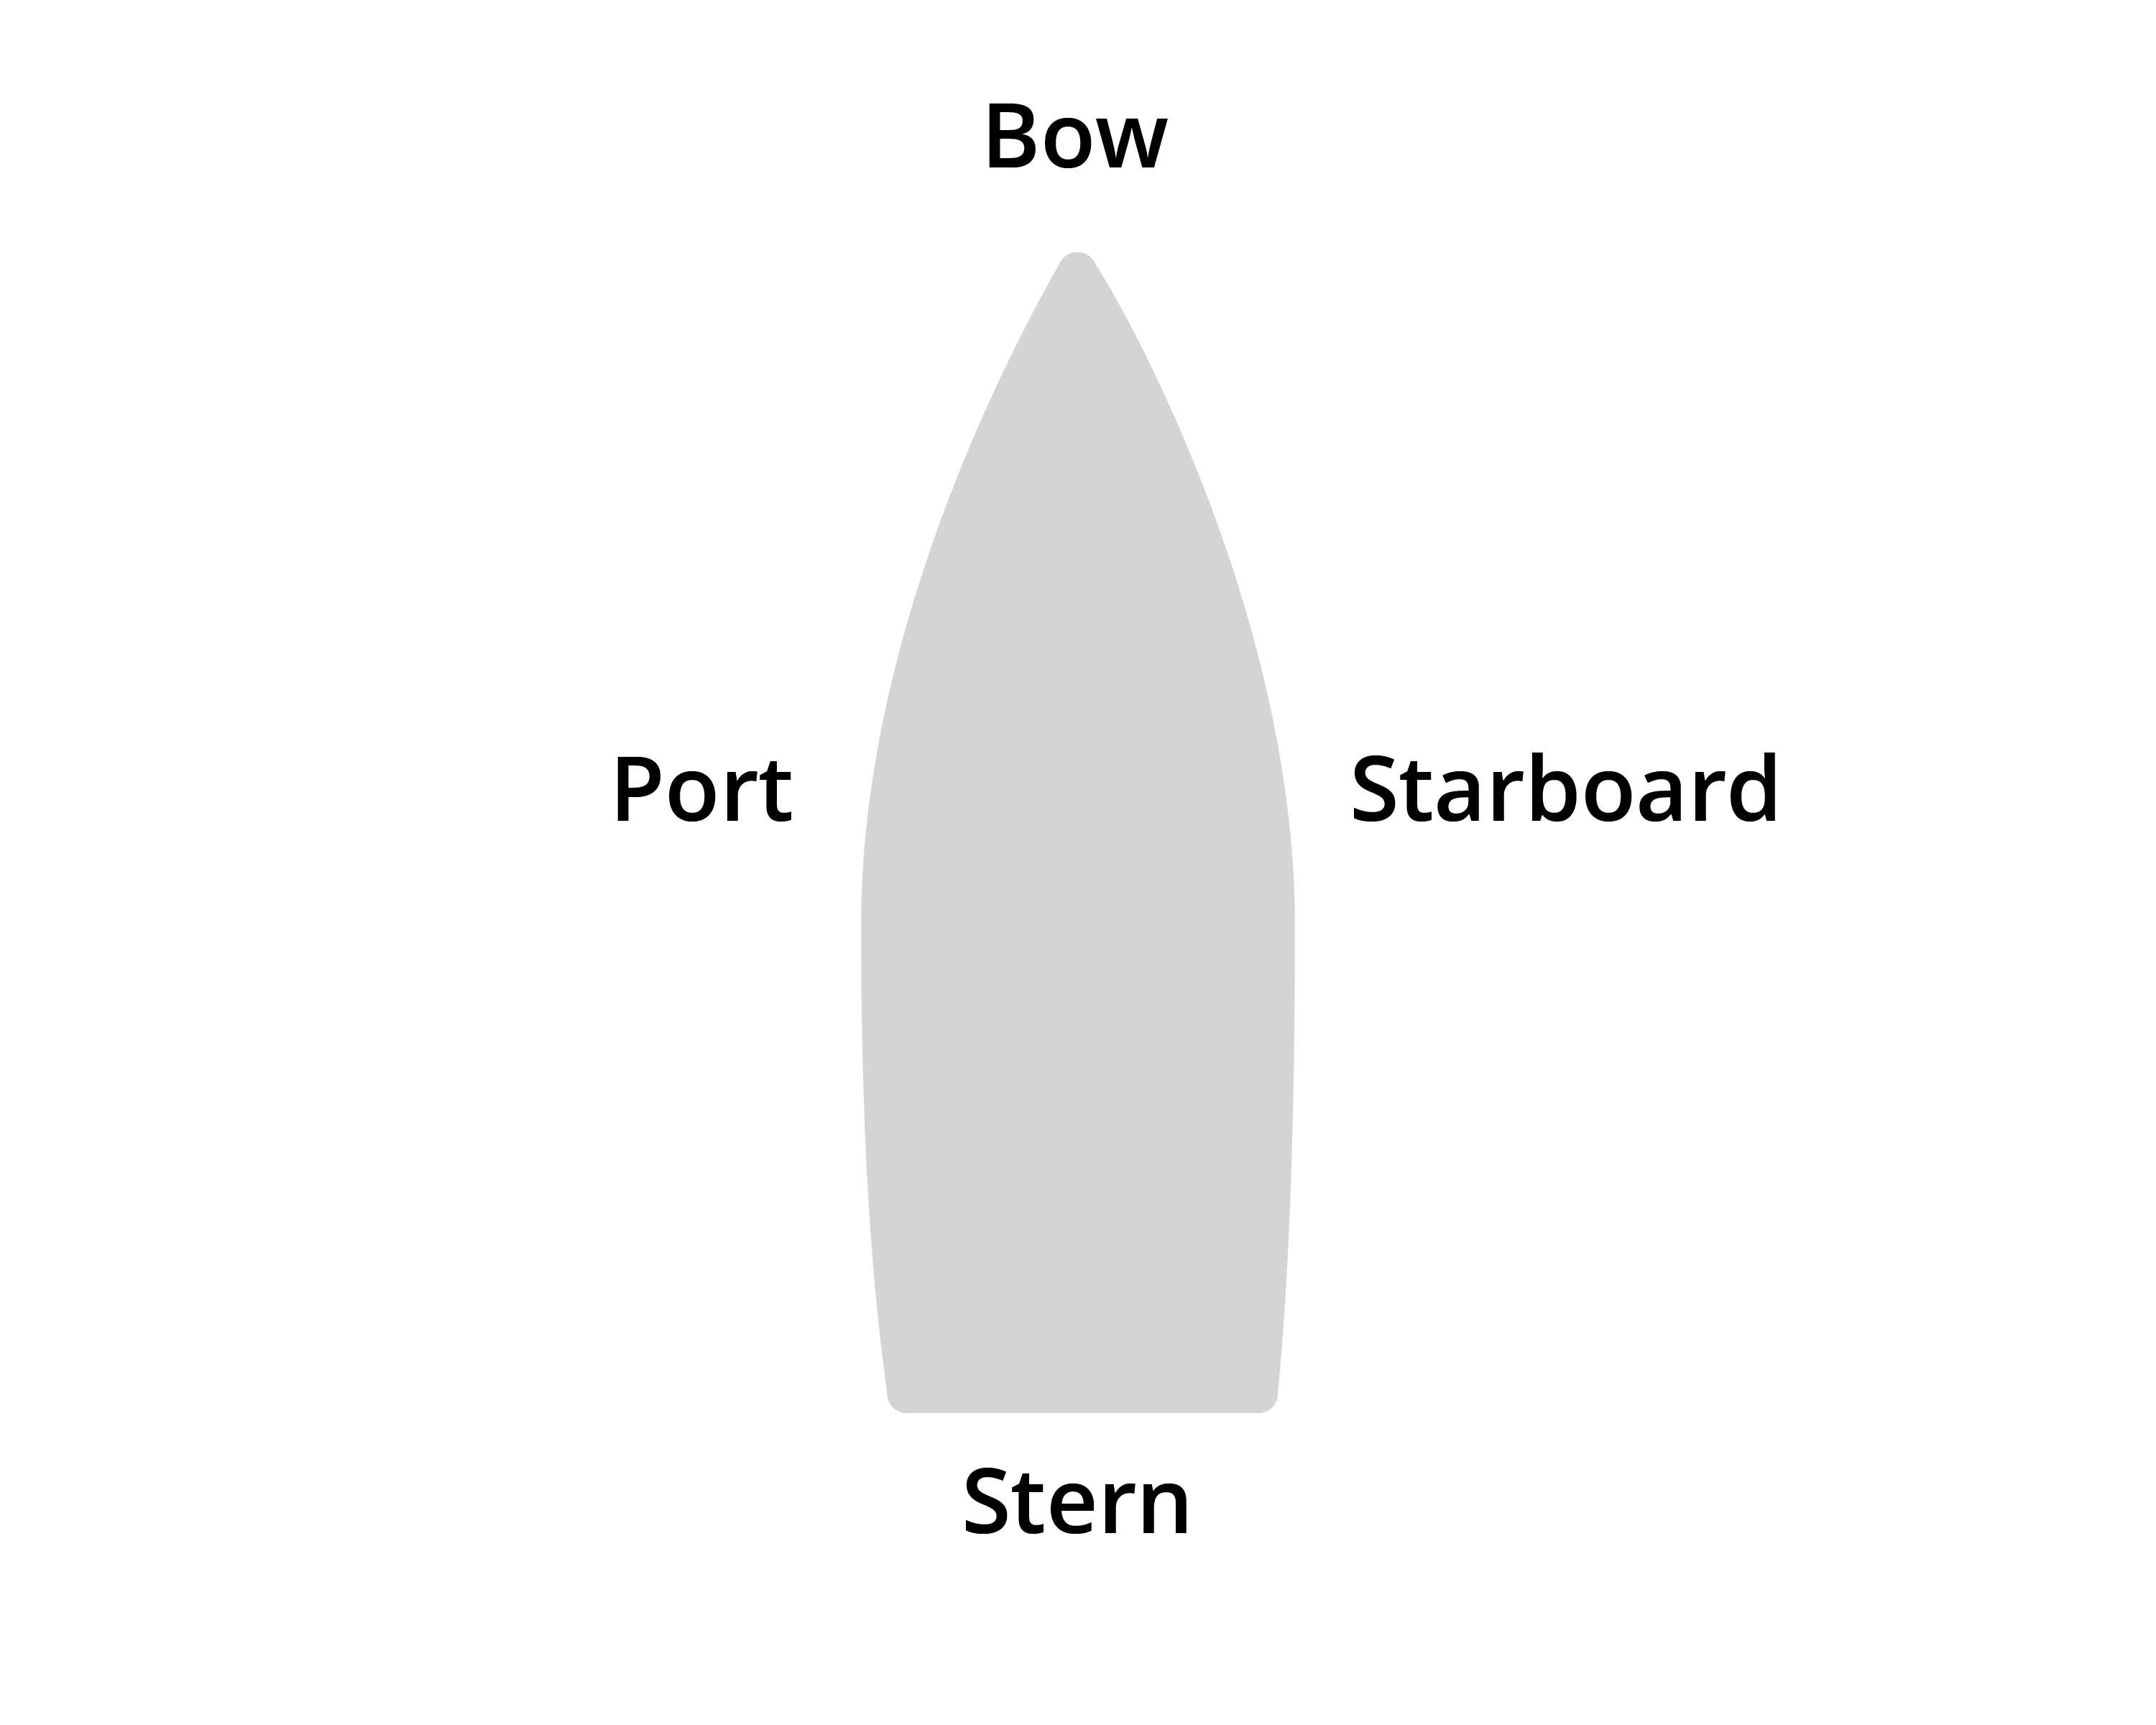
\includegraphics[width=.75\textwidth]{bowStern.png}

There are several different ways that boats are propelled:

\begin{itemize}


\item A motor turns a screw in the water, as in a motorboat. The screw is known as a \newterm{propeller}.

\item A human pushes the water with a stick.  If the stick is attached to the boat with a pivot (as in a rowboat) it is an \newterm{oar}.  If the blade is not attached to the boat (as in a canoe), it is a \newterm{paddle}.

\item A human pushes the ground beneath the water with a long pole. These boats are called \newterm{punts}, and are mainly used in more shallow waters where an oar or a paddle would be less convenient.

\item The wind pushes the boat,  as in a sailboat. The sails are held up by a \newterm{mast}.

\item Some boats have a big fan that pushes the boat.  These are called \newterm{airboats}.   Airboats are not the most efficient boats,  but they can travel
on waterways with water just a couple of inches deep.

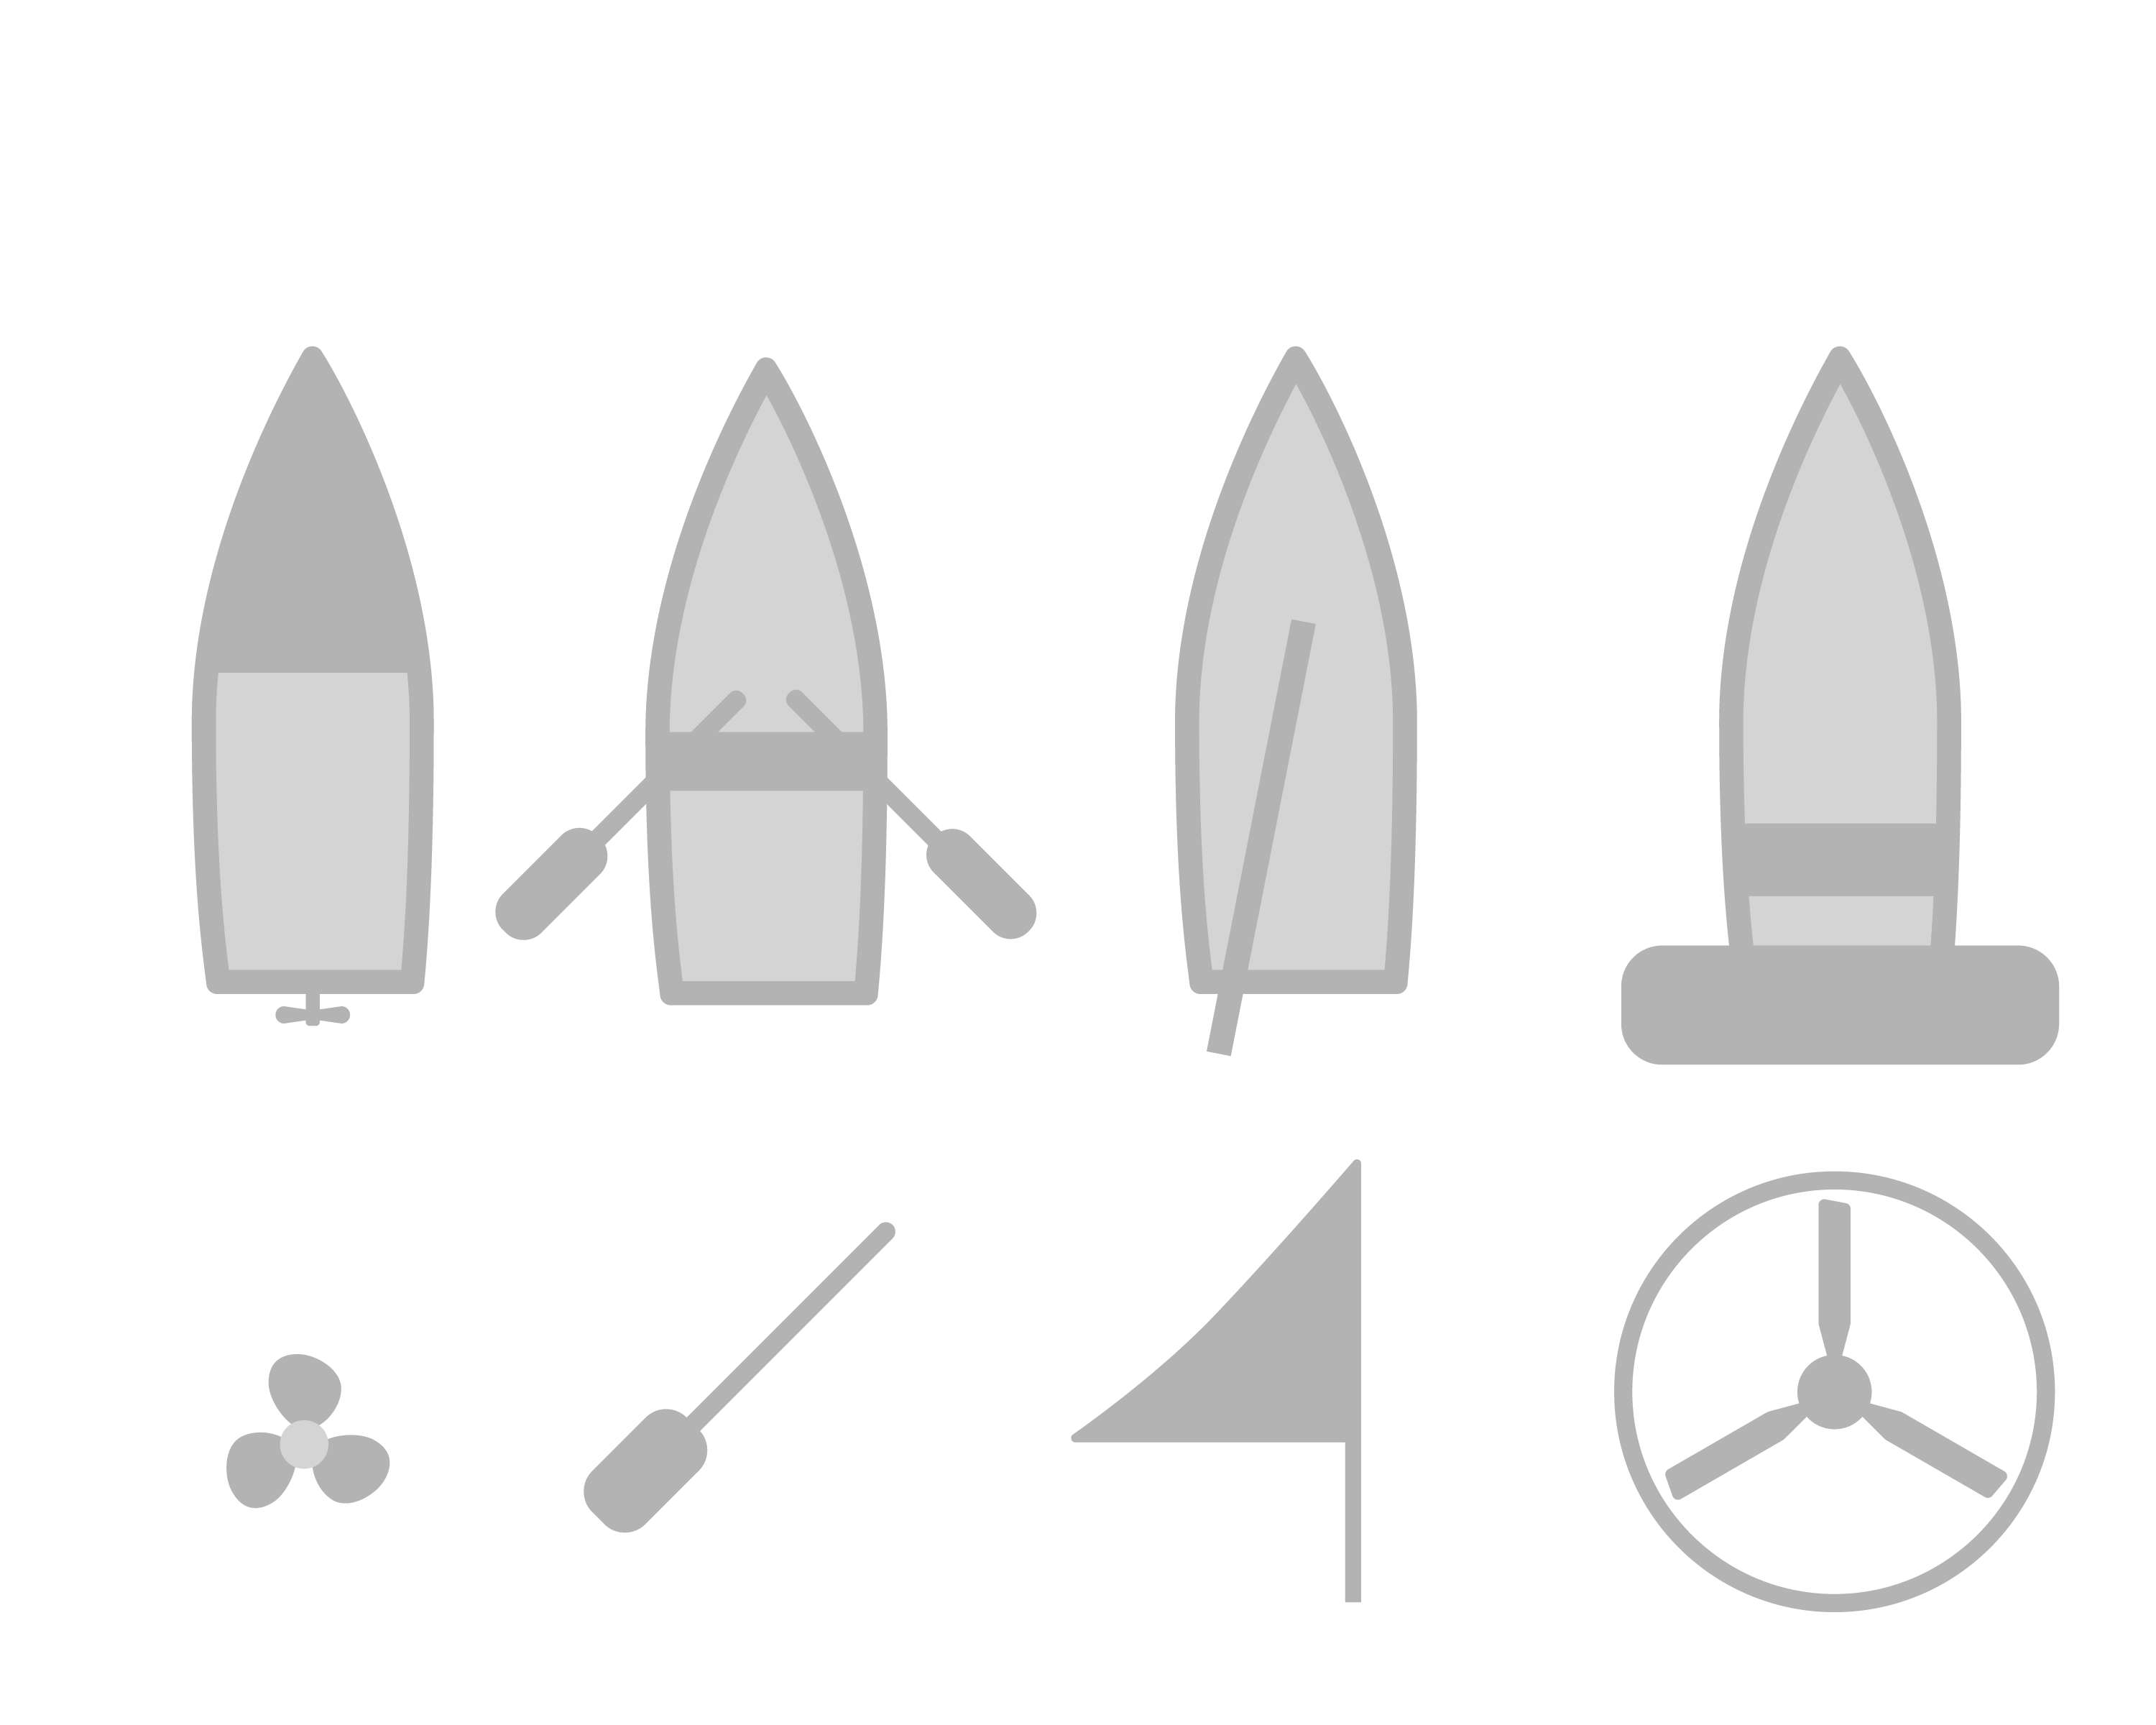
\includegraphics[width=.75\textwidth]{boatTypes.png}


\end{itemize}

In the terms of physics, each of these method provide a \newterm{thrust vector} which is applied to the boat at a particular place and in a particular direction.

The speed of a boat is usually measured in \newterm{knots}. 1 knot is 1 nautical mile per hour, or 1.852 km per hour.

\section{Why Boats Float Upright}

Early in this sequence, we discussed buoyancy as a quantity. The magnitude of the buoyant force is equivalent to the weight of the liquid displaced.

We can also talk about the direction of the buoyant force: buoyancy pushes in the opposite direction as gravity.

How do we design boats so that they don't flip over?

\subsection{Center of Buoyancy}

Let's say you have a rowboat. If you push down on point on the floor near the front, the front of the boat will go down and the back of the boat will rise. In other words, the boat will rotate in the direction you are pushing. 
Likewise, if you push on the floor near the back of the boat, the back will sink a little lower and the front will rise. However, there is a place, near the center of the boat, where if you push down, the boat will not rotate at all; it will simply sink a little lower
in the water. That point is known as the \newterm{center of buoyancy}.


How can we calculate the center of buoyancy?  Imagine the shape of the water that was displaced by the boat. Now imagine that shape filled with water. The center of mass of that water is the center of buoyancy of the boat.

\subsection{Center of Mass}

Your boat and everything in it can be thought of as one object.  That object has a center of mass. If you found the center of mass, you could balance the whole boat on it.

In a boat,  if you move your body from the center of the boat to once side, you will have moved the center of mass. The boat will lean in that direction, which will change the center of buoyancy. 

If you imagine a line is parallel to the force of gravity that passes through the center of mass of your boat, the boat will continue to increase its lean until
the center of buoyancy is on that line.  

If water comes over the sides of the boat before the center of gravity and center of buoyancy align, your boat will sink.

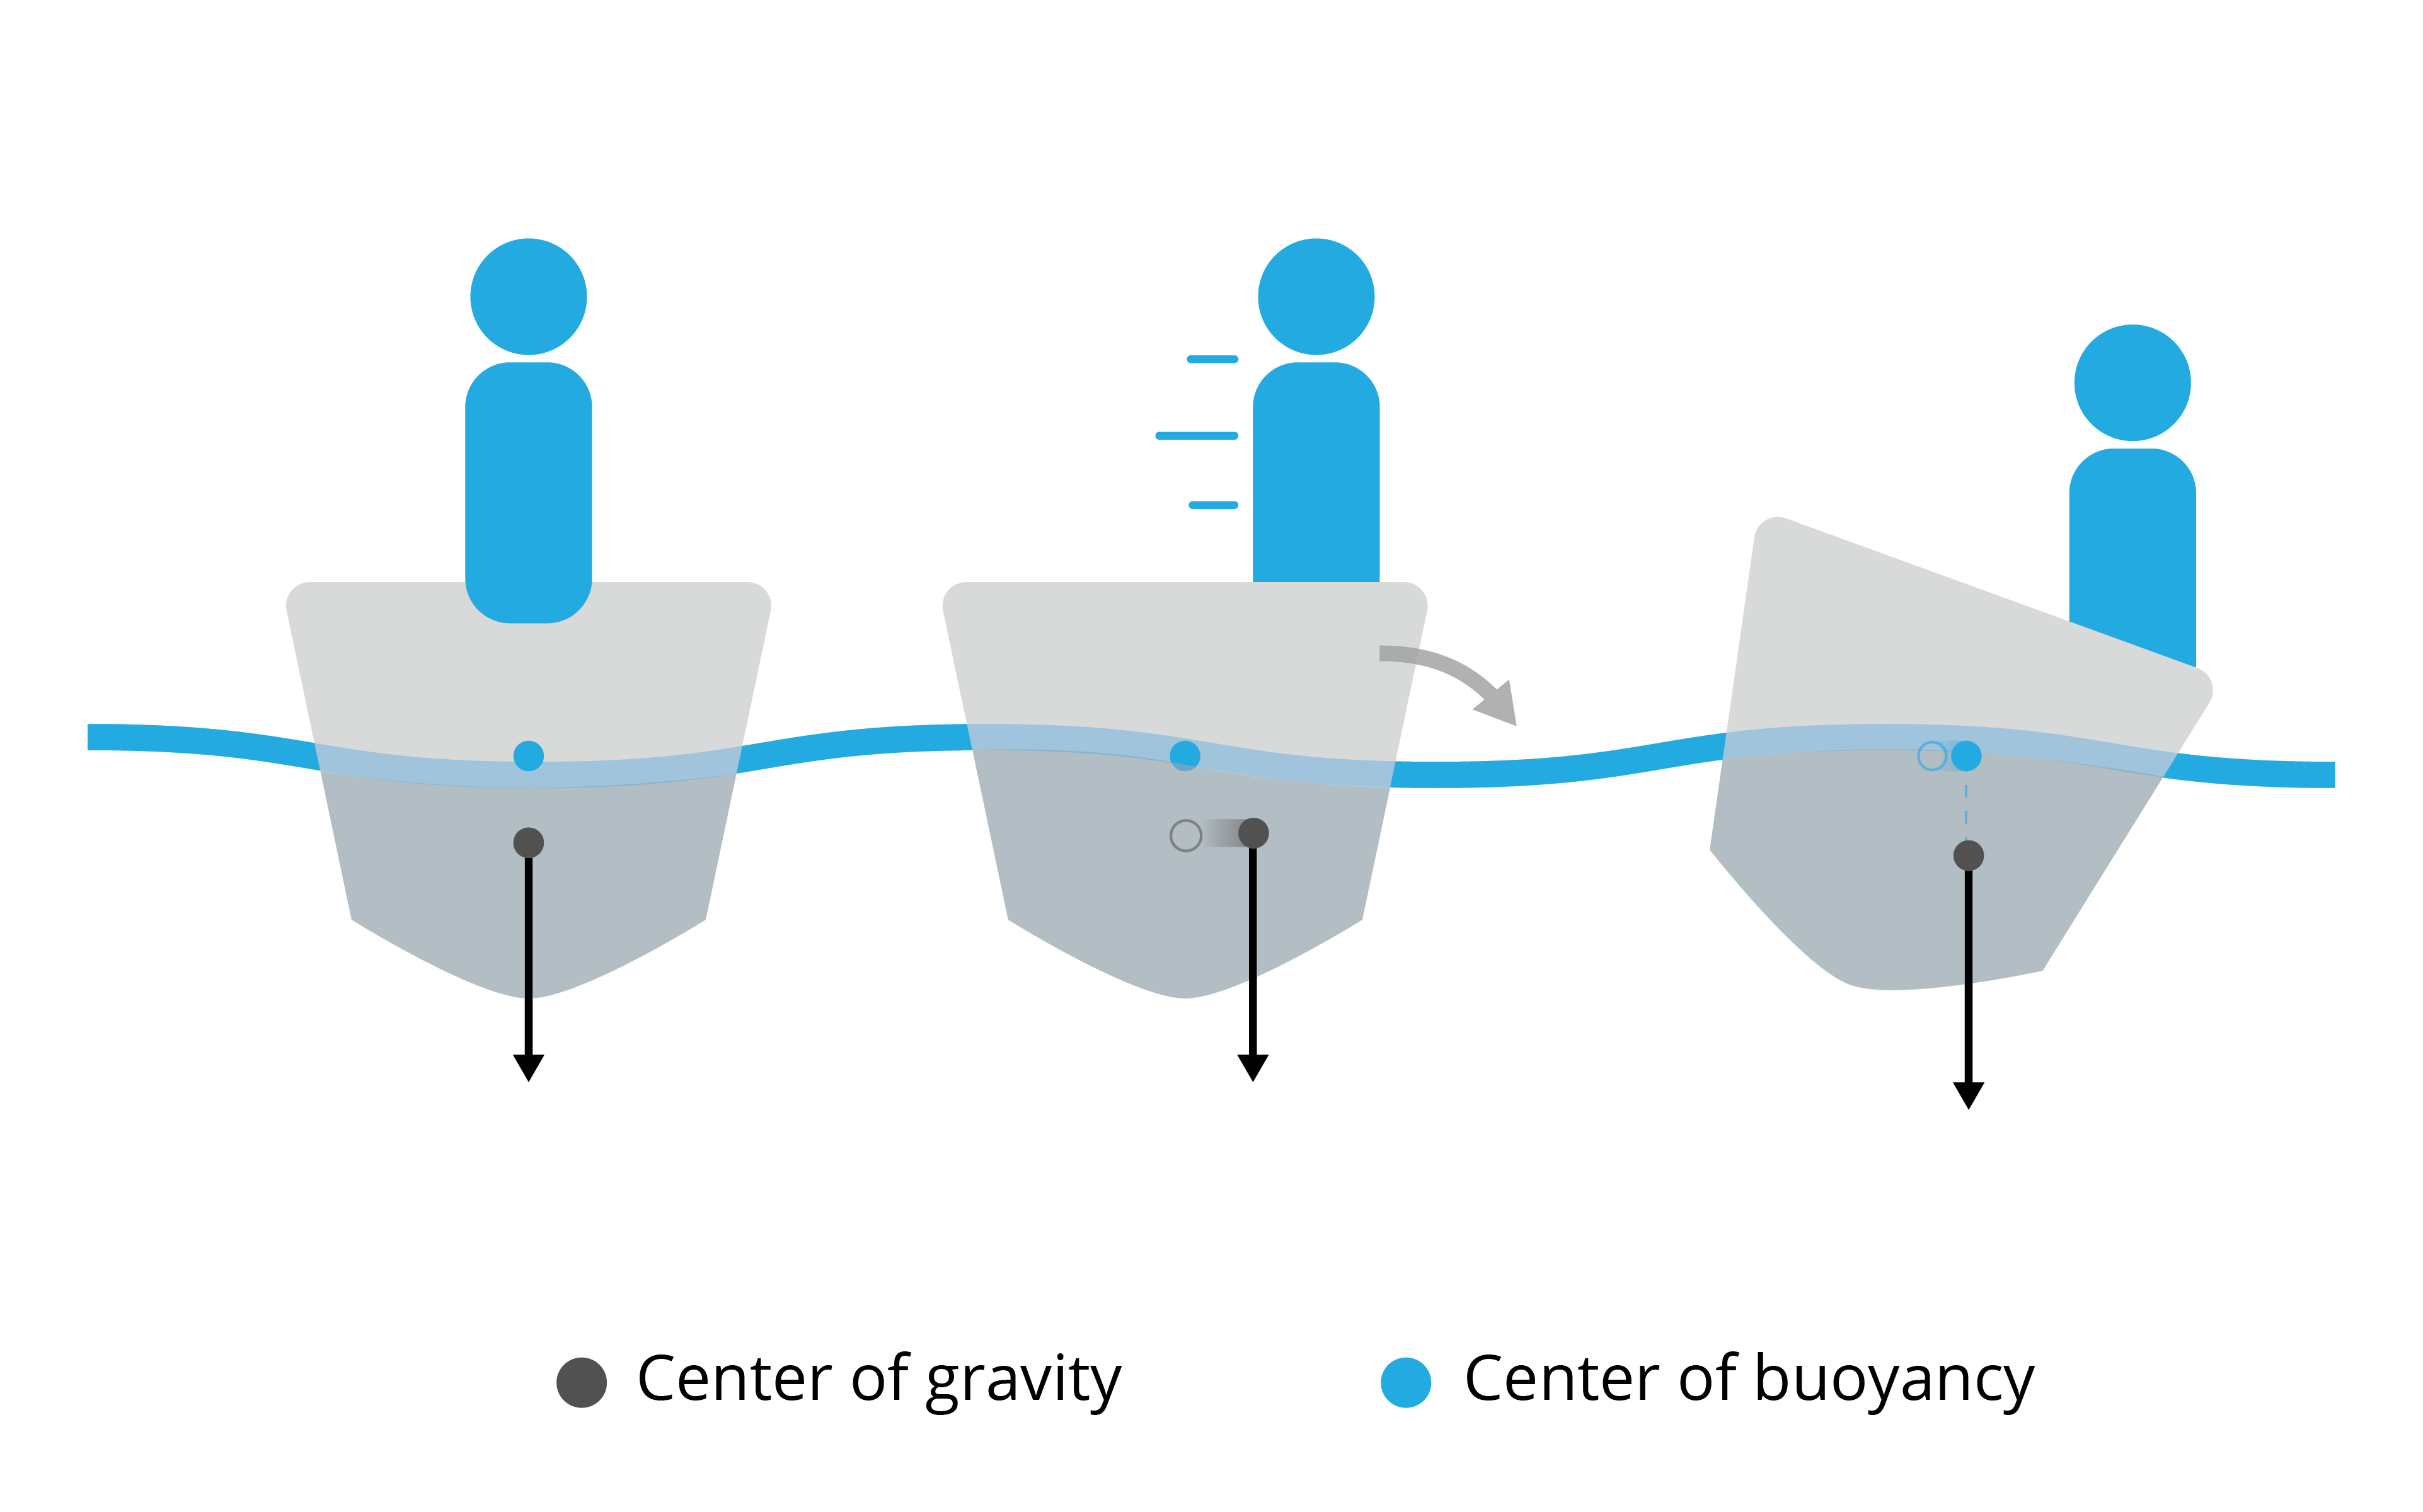
\includegraphics[width=.75\textwidth]{cgcm.png}


\section{Center of Lateral Resistance}

It isn't enough for a boat to float --- for a boat to be useful,  it must also be able to travel in a straight line.

Imagine that you are standing knee-deep in a lake next to a canoe.  If you push the front of the canoe away from you,  it will rotate --- the back end will actually
swing toward you. There is a point near the middle of the canoe where if you push it will not rotate in either direction --- the boat will just slide sideways.  This point is known as the \newterm{center of lateral resistance}.

The trick to making a boat travel in a straight line is to make sure that the line that contains the thrust vector passes through the center of lateral resistance.

An outboard motor allows you to direct the thrust vector. When the line of thrust passes the center of lateral resistance on the starboard side of the center of lateral resistance, the boat turns toward the port side.

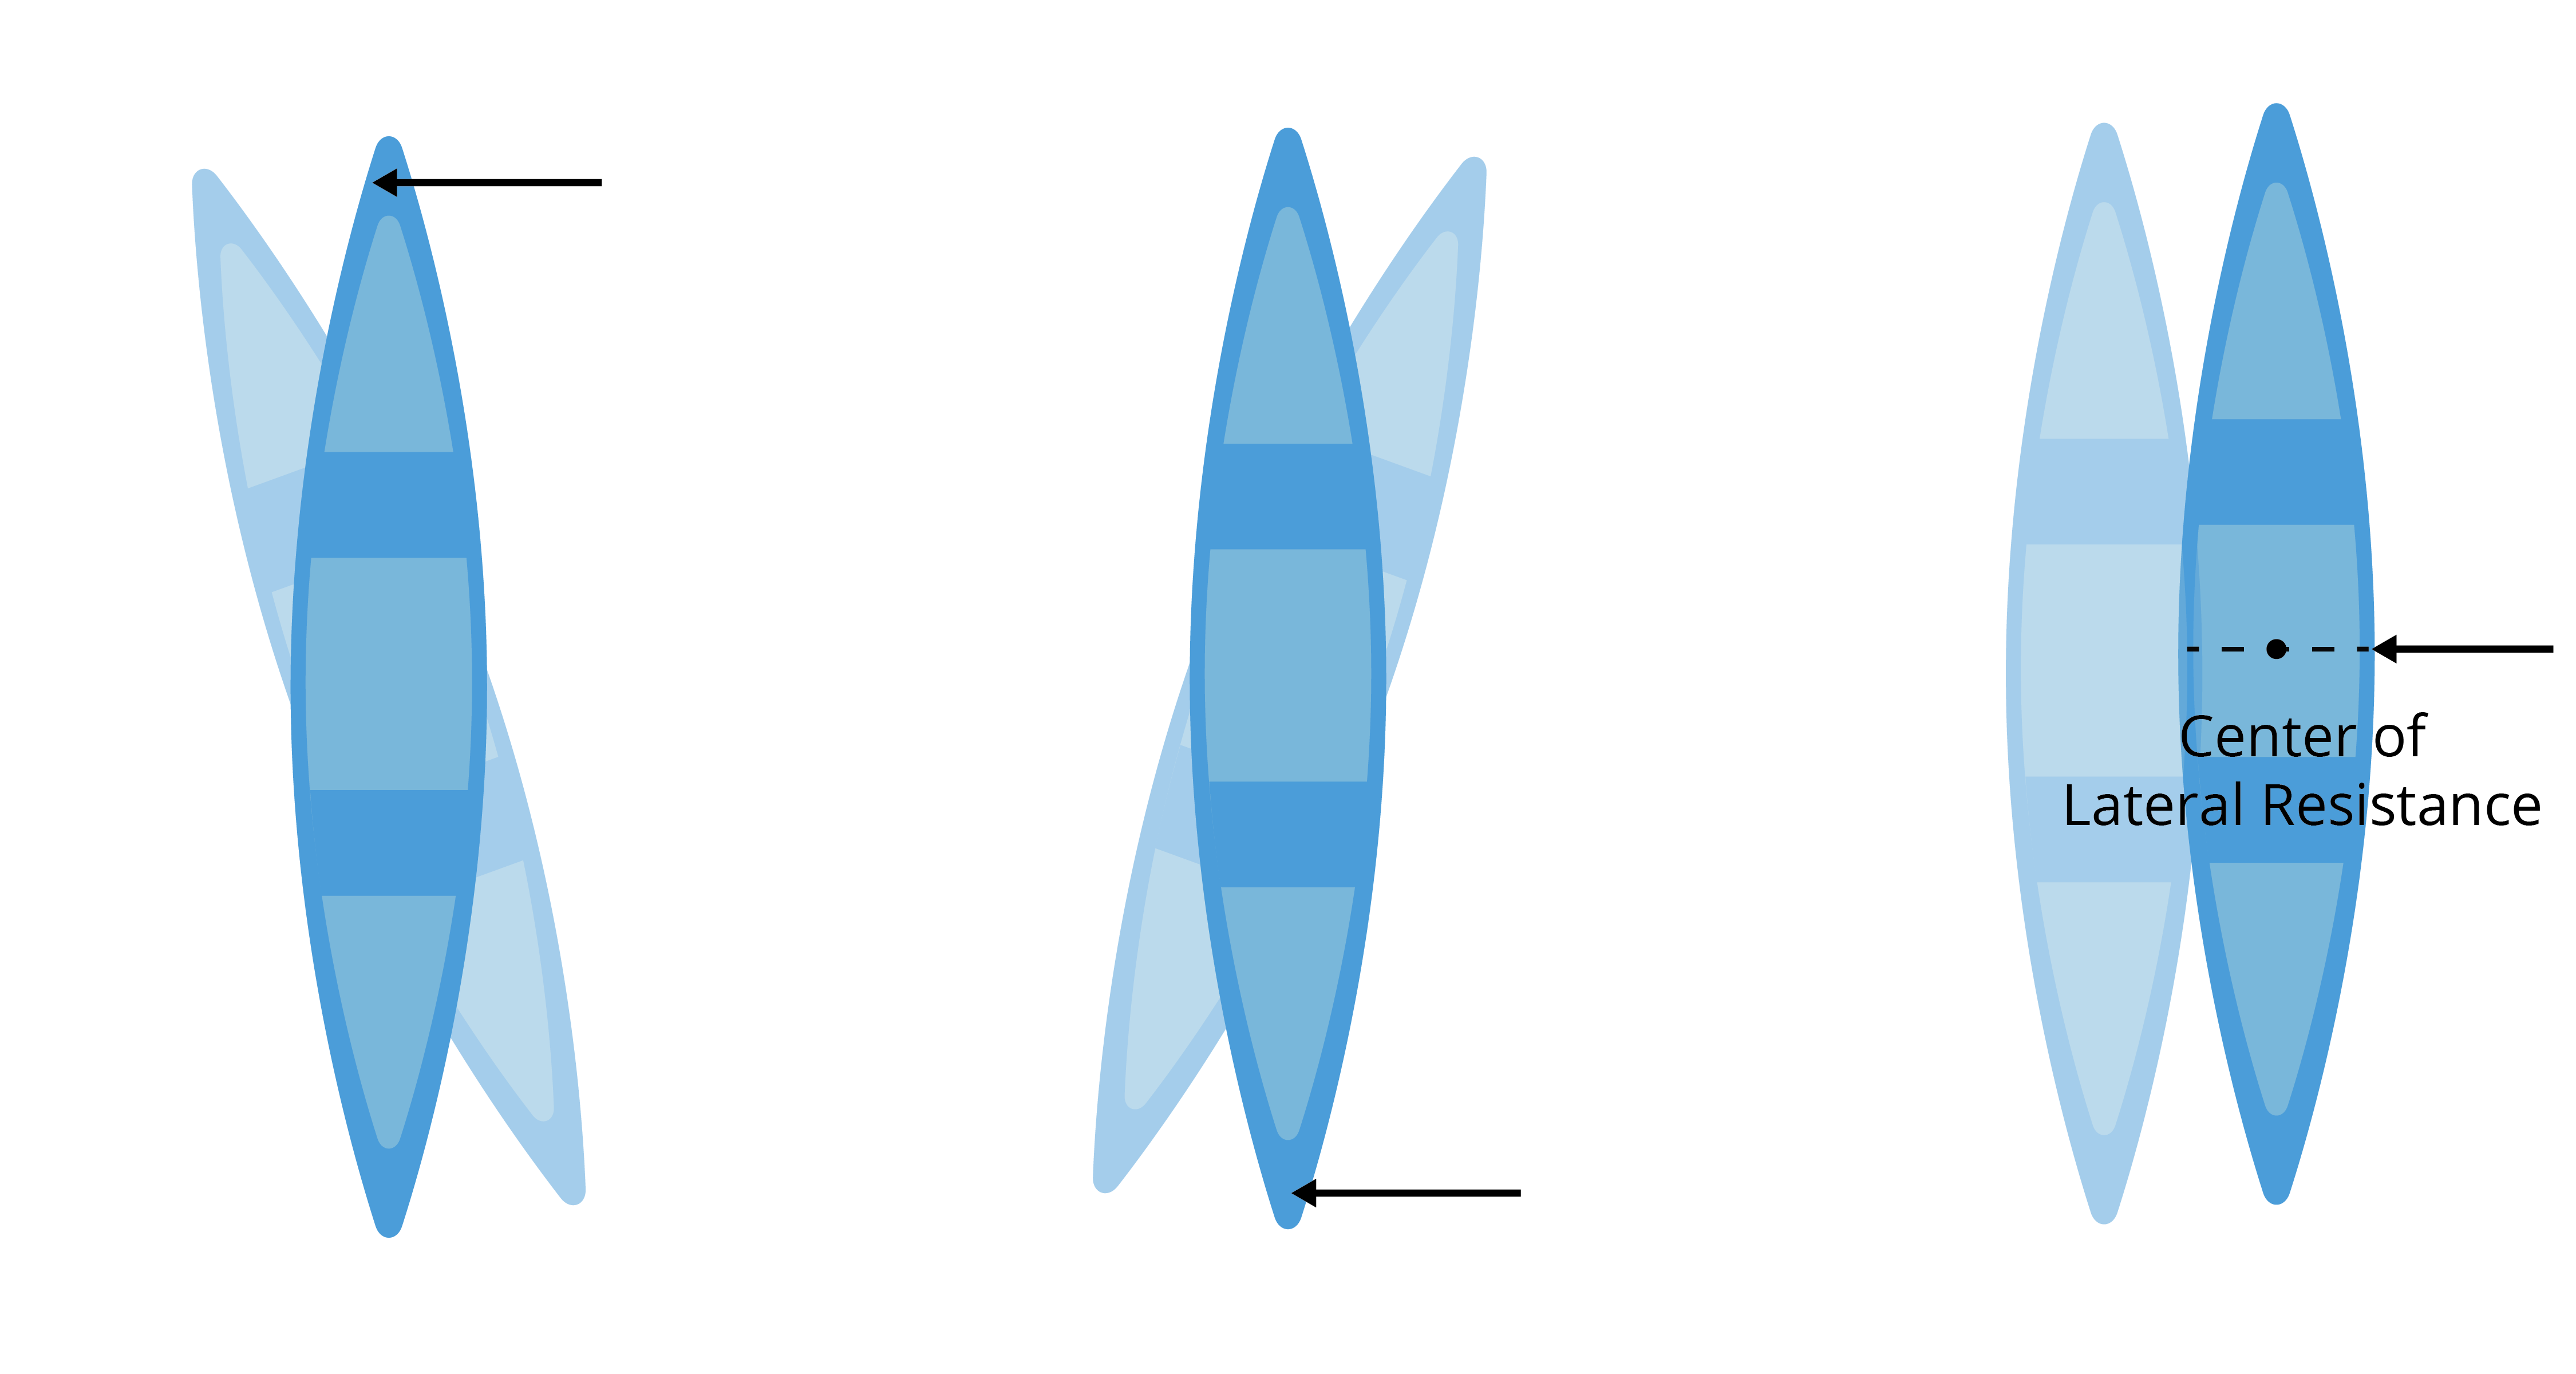
\includegraphics[width=.75\textwidth]{lateralResistance.png}


\section{Steering with a Rudder}
 
While outboard motors and airboats let you direct the thrust vector,  most boats have a \newterm{rudder}.  The rudder is a blade on a pivot near the back of 
the boat. The angle of the rudder can be adjusted so that water rushing past it gets pushed to one side or the other.

According to Newton's third law,  when the water gets pushed to the left,  the back of the boat gets pushed (with the same force) to the right.  This causes the boat to rotate around its center of lateral resistance.

Note that a rudder only works when the boat is passing through the water. 

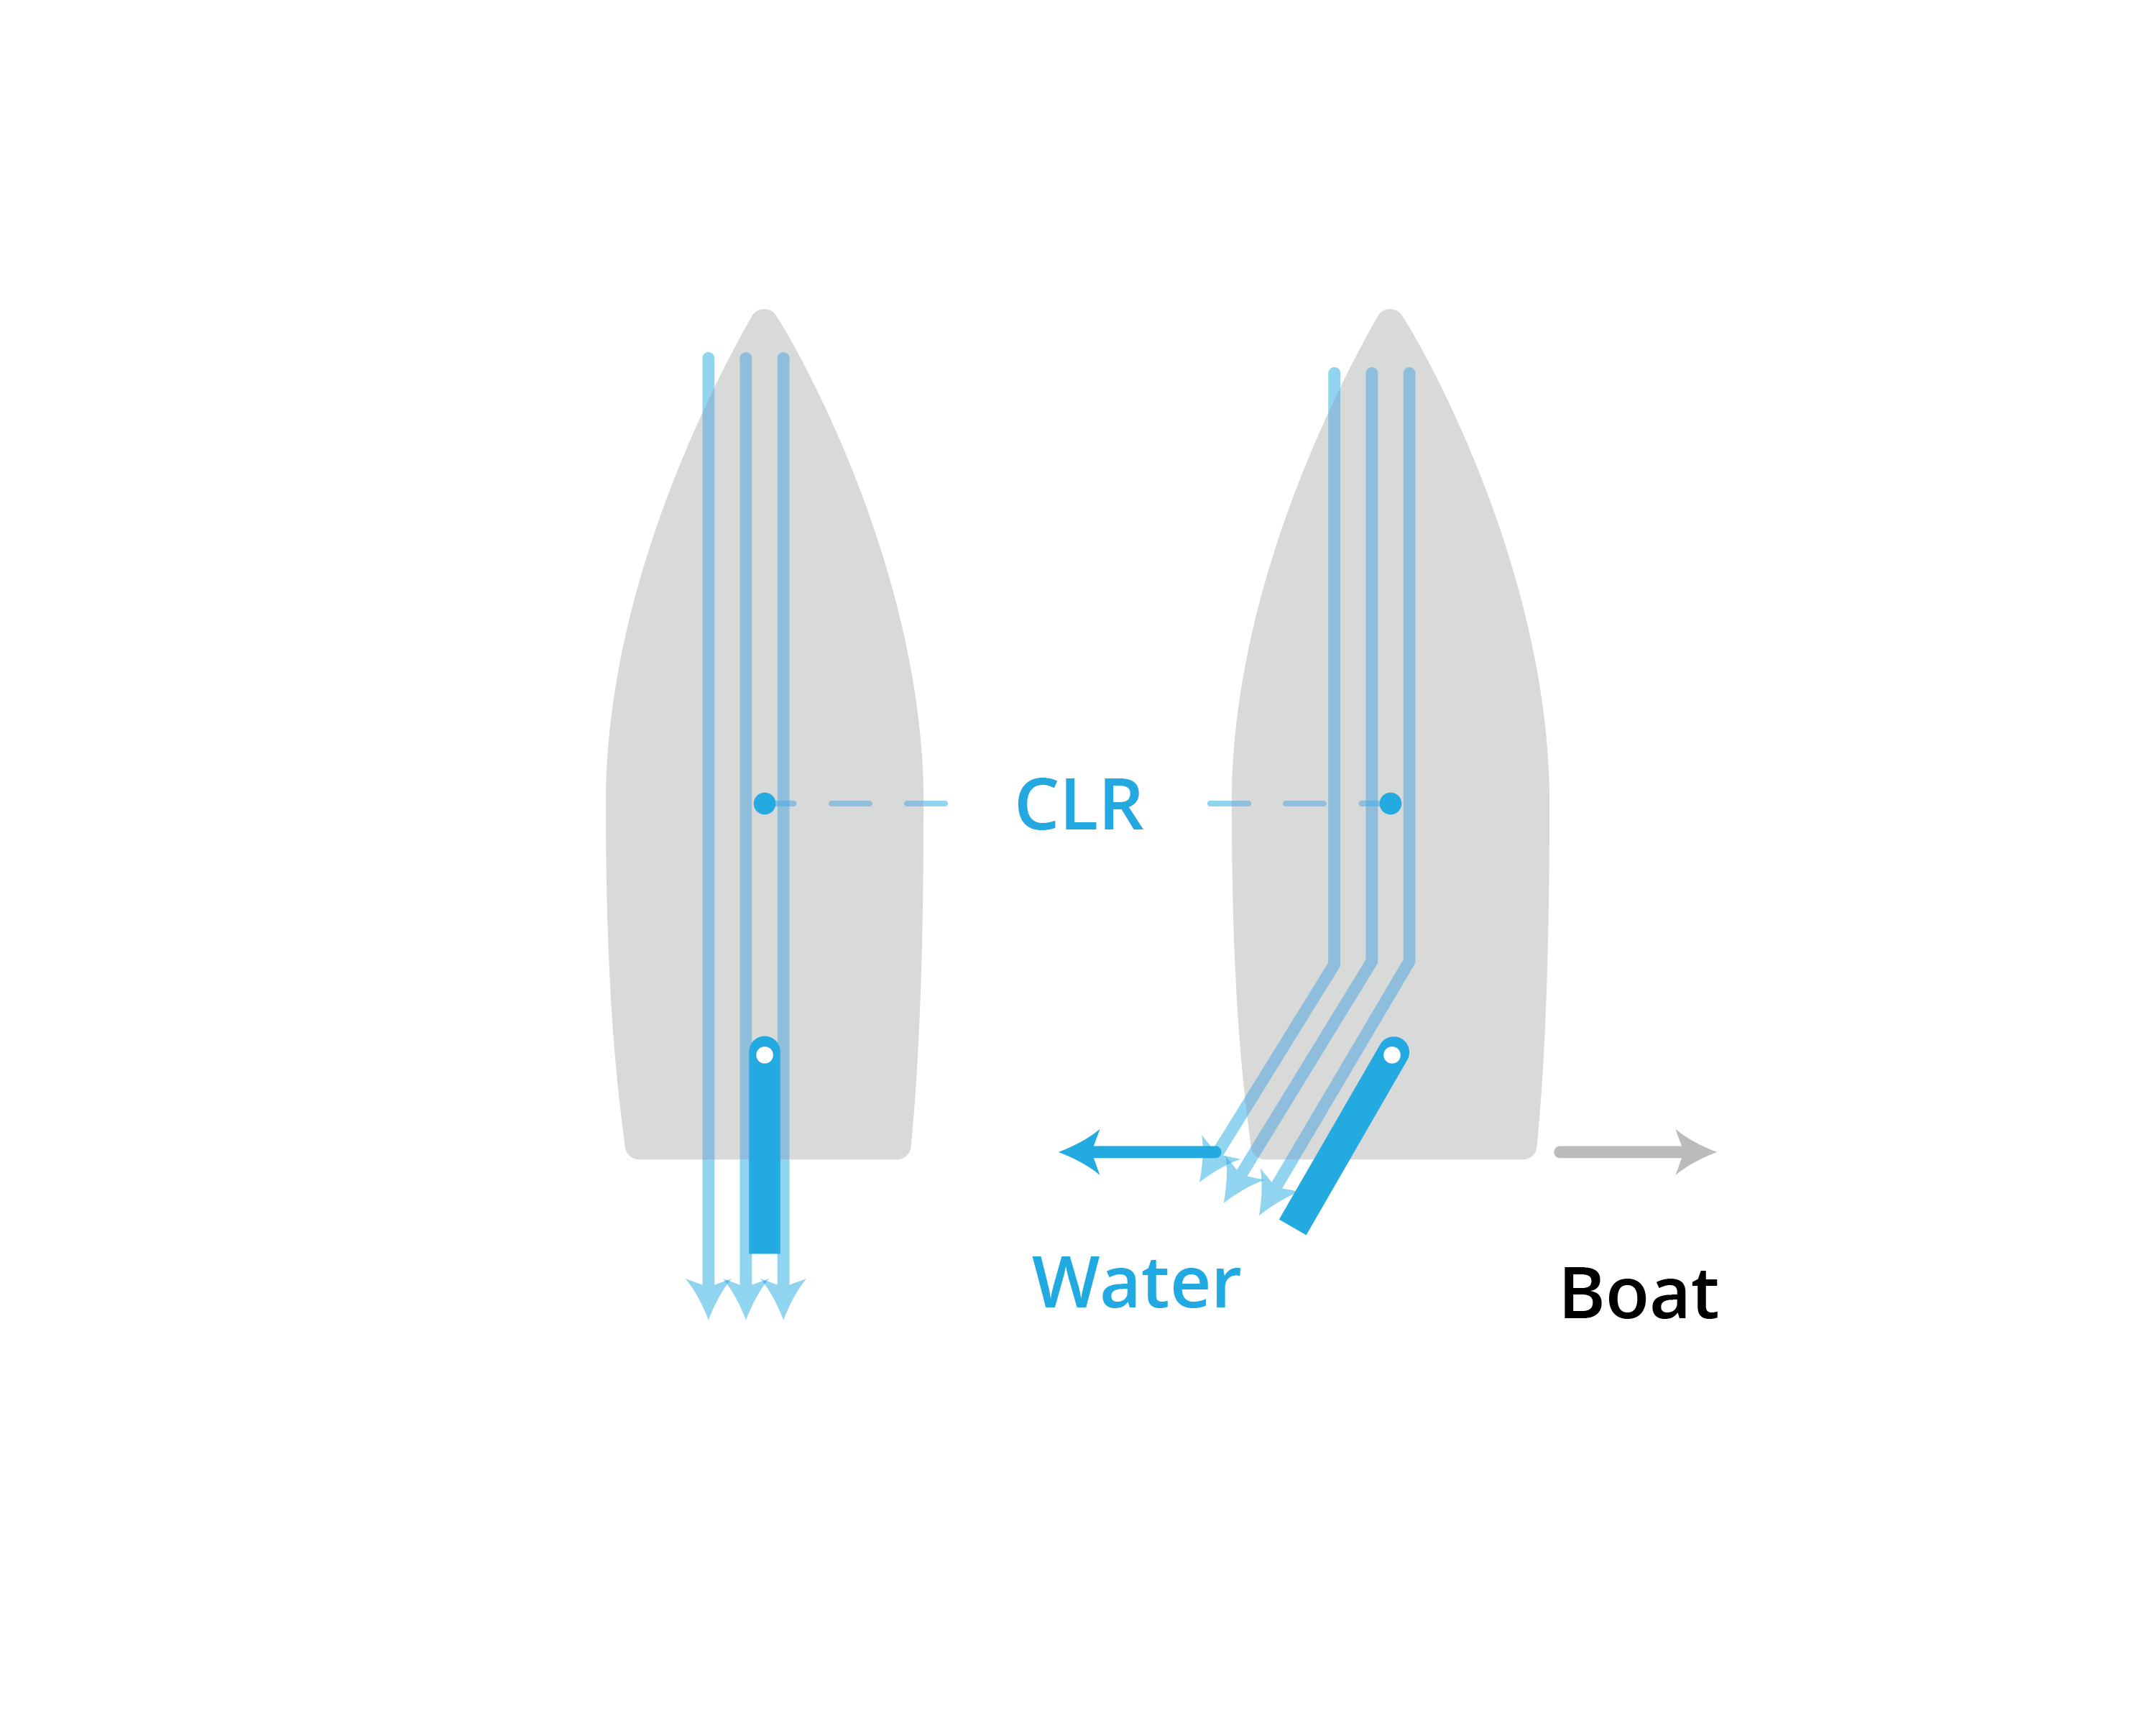
\includegraphics[width=.75\textwidth]{rudder.png}


\section{Boat Length and Resistance}

FIXME: Write about wave length,  boat length, and Froude number.






